% Figure 2: one 2x2 pooling window, the exact range of the maximum and the outputs of the admissible maxima.
% Compile with pdflatex; the PDF is included in main.tex at its natural size.
\documentclass[tikz,border=2pt]{standalone}
\usepackage[T1]{fontenc}
\usepackage{lmodern}
\usepackage{amsmath,amssymb}
\usetikzlibrary{arrows.meta}
\definecolor{lattice}{HTML}{2A78D6}
\definecolor{lexb}{HTML}{EB6834}   % Lex2
\definecolor{lexa}{HTML}{1BAF7A}   % Lex1
\definecolor{xy}{HTML}{B5438F}     % Xu--Yager
\definecolor{ink}{HTML}{1A1A1A}
\definecolor{muted}{HTML}{6B6B6B}
\begin{document}
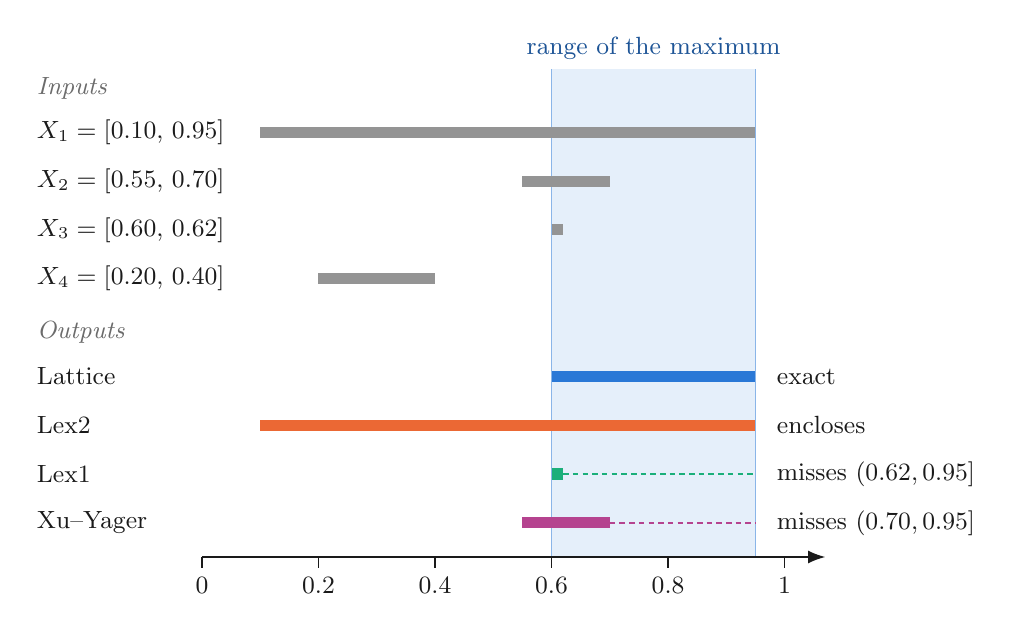
\begin{tikzpicture}[x=7.4cm,y=0.62cm,font=\small,text=ink,draw=ink]
  % the range of the maximum, as a band behind everything
  \fill[lattice!12] (0.60,-0.1) rectangle (0.95,9.9);
  \draw[lattice!55,line width=0.4pt] (0.60,-0.1) -- (0.60,9.9) (0.95,-0.1) -- (0.95,9.9);
  \node[anchor=south,lattice!70!black] at (0.775,9.9) {range of the maximum};
  % axis
  \draw[-{Latex[length=2.2mm]},line width=0.6pt] (0,-0.1) -- (1.07,-0.1);
  \foreach \t in {0,0.2,0.4,0.6,0.8,1} {\draw[line width=0.6pt] (\t,-0.1) -- (\t,-0.32) node[below] {$\t$};}
  % inputs
  \node[anchor=west,muted] at (-0.3,9.5) {\emph{Inputs}};
  \foreach \l/\u/\y/\n in {0.10/0.95/8.6/1, 0.55/0.70/7.6/2, 0.60/0.62/6.6/3, 0.20/0.40/5.6/4} {
    \draw[line width=4pt,black!42] (\l,\y) -- (\u,\y);
    \node[anchor=west] at (-0.3,\y) {$X_\n=[\l,\,\u]$};
  }
  % outputs
  \node[anchor=west,muted] at (-0.3,4.5) {\emph{Outputs}};
  \draw[line width=4pt,lattice] (0.60,3.6) -- (0.95,3.6);
  \node[anchor=west] at (-0.3,3.6) {Lattice};
  \draw[line width=4pt,lexb] (0.10,2.6) -- (0.95,2.6);
  \node[anchor=west] at (-0.3,2.6) {Lex2};
  \draw[line width=4pt,lexa] (0.60,1.6) -- (0.62,1.6);
  \node[anchor=west] at (-0.3,1.6) {Lex1};
  \draw[line width=4pt,xy] (0.55,0.6) -- (0.70,0.6);
  \node[anchor=west] at (-0.3,0.6) {Xu--Yager};
  % what the unsound outputs miss
  \draw[lexa,line width=0.8pt,dash pattern=on 2pt off 1.5pt] (0.62,1.6) -- (0.95,1.6);
  \draw[xy,line width=0.8pt,dash pattern=on 2pt off 1.5pt] (0.70,0.6) -- (0.95,0.6);
  \node[anchor=west] at (0.97,3.6) {exact};
  \node[anchor=west] at (0.97,2.6) {encloses};
  \node[anchor=west] at (0.97,1.6) {misses $(0.62,0.95]$};
  \node[anchor=west] at (0.97,0.6) {misses $(0.70,0.95]$};
\end{tikzpicture}
\end{document}
